\section{Own Contribution}
In this section we present four different case studies to answer our research questions. We begin with presenting
\UH{} as it is the project which focus our efforts of improvement on. It is followed by \textit{Battle for
Wesnoth}, \textit{Mega Glest} and \textit{0 A.D.}.
The results are then evaluated and transferred to \UH{}.

\subsection{Unknown Horizons}
\UH{} as described on the project website:
\begin{quote}
\UH{} is a 2D realtime strategy simulation with an emphasis on economy and city building. Expand your small settlement to a strong and wealthy colony, collect taxes and supply your inhabitants with valuable goods. Increase your power with a well balanced economy and with strategic trade and diplomacy.
\end{quote}

\subsubsection{RQ1}
\UH{} uses a largely inheritance based approach to describe ingame objects. As the game is programmed using
the Python\footnote{Python website: \url{http://www.python.org}} programming language it is possible to use multiple
inheritance. The project makes great use of this ability, resulting in large inheritance trees. To illustrate this we
have generated an inheritance diagramm for the \textit{Settler} class in \figref{fig:settleruml}. 
\begin{figure}[!htb]
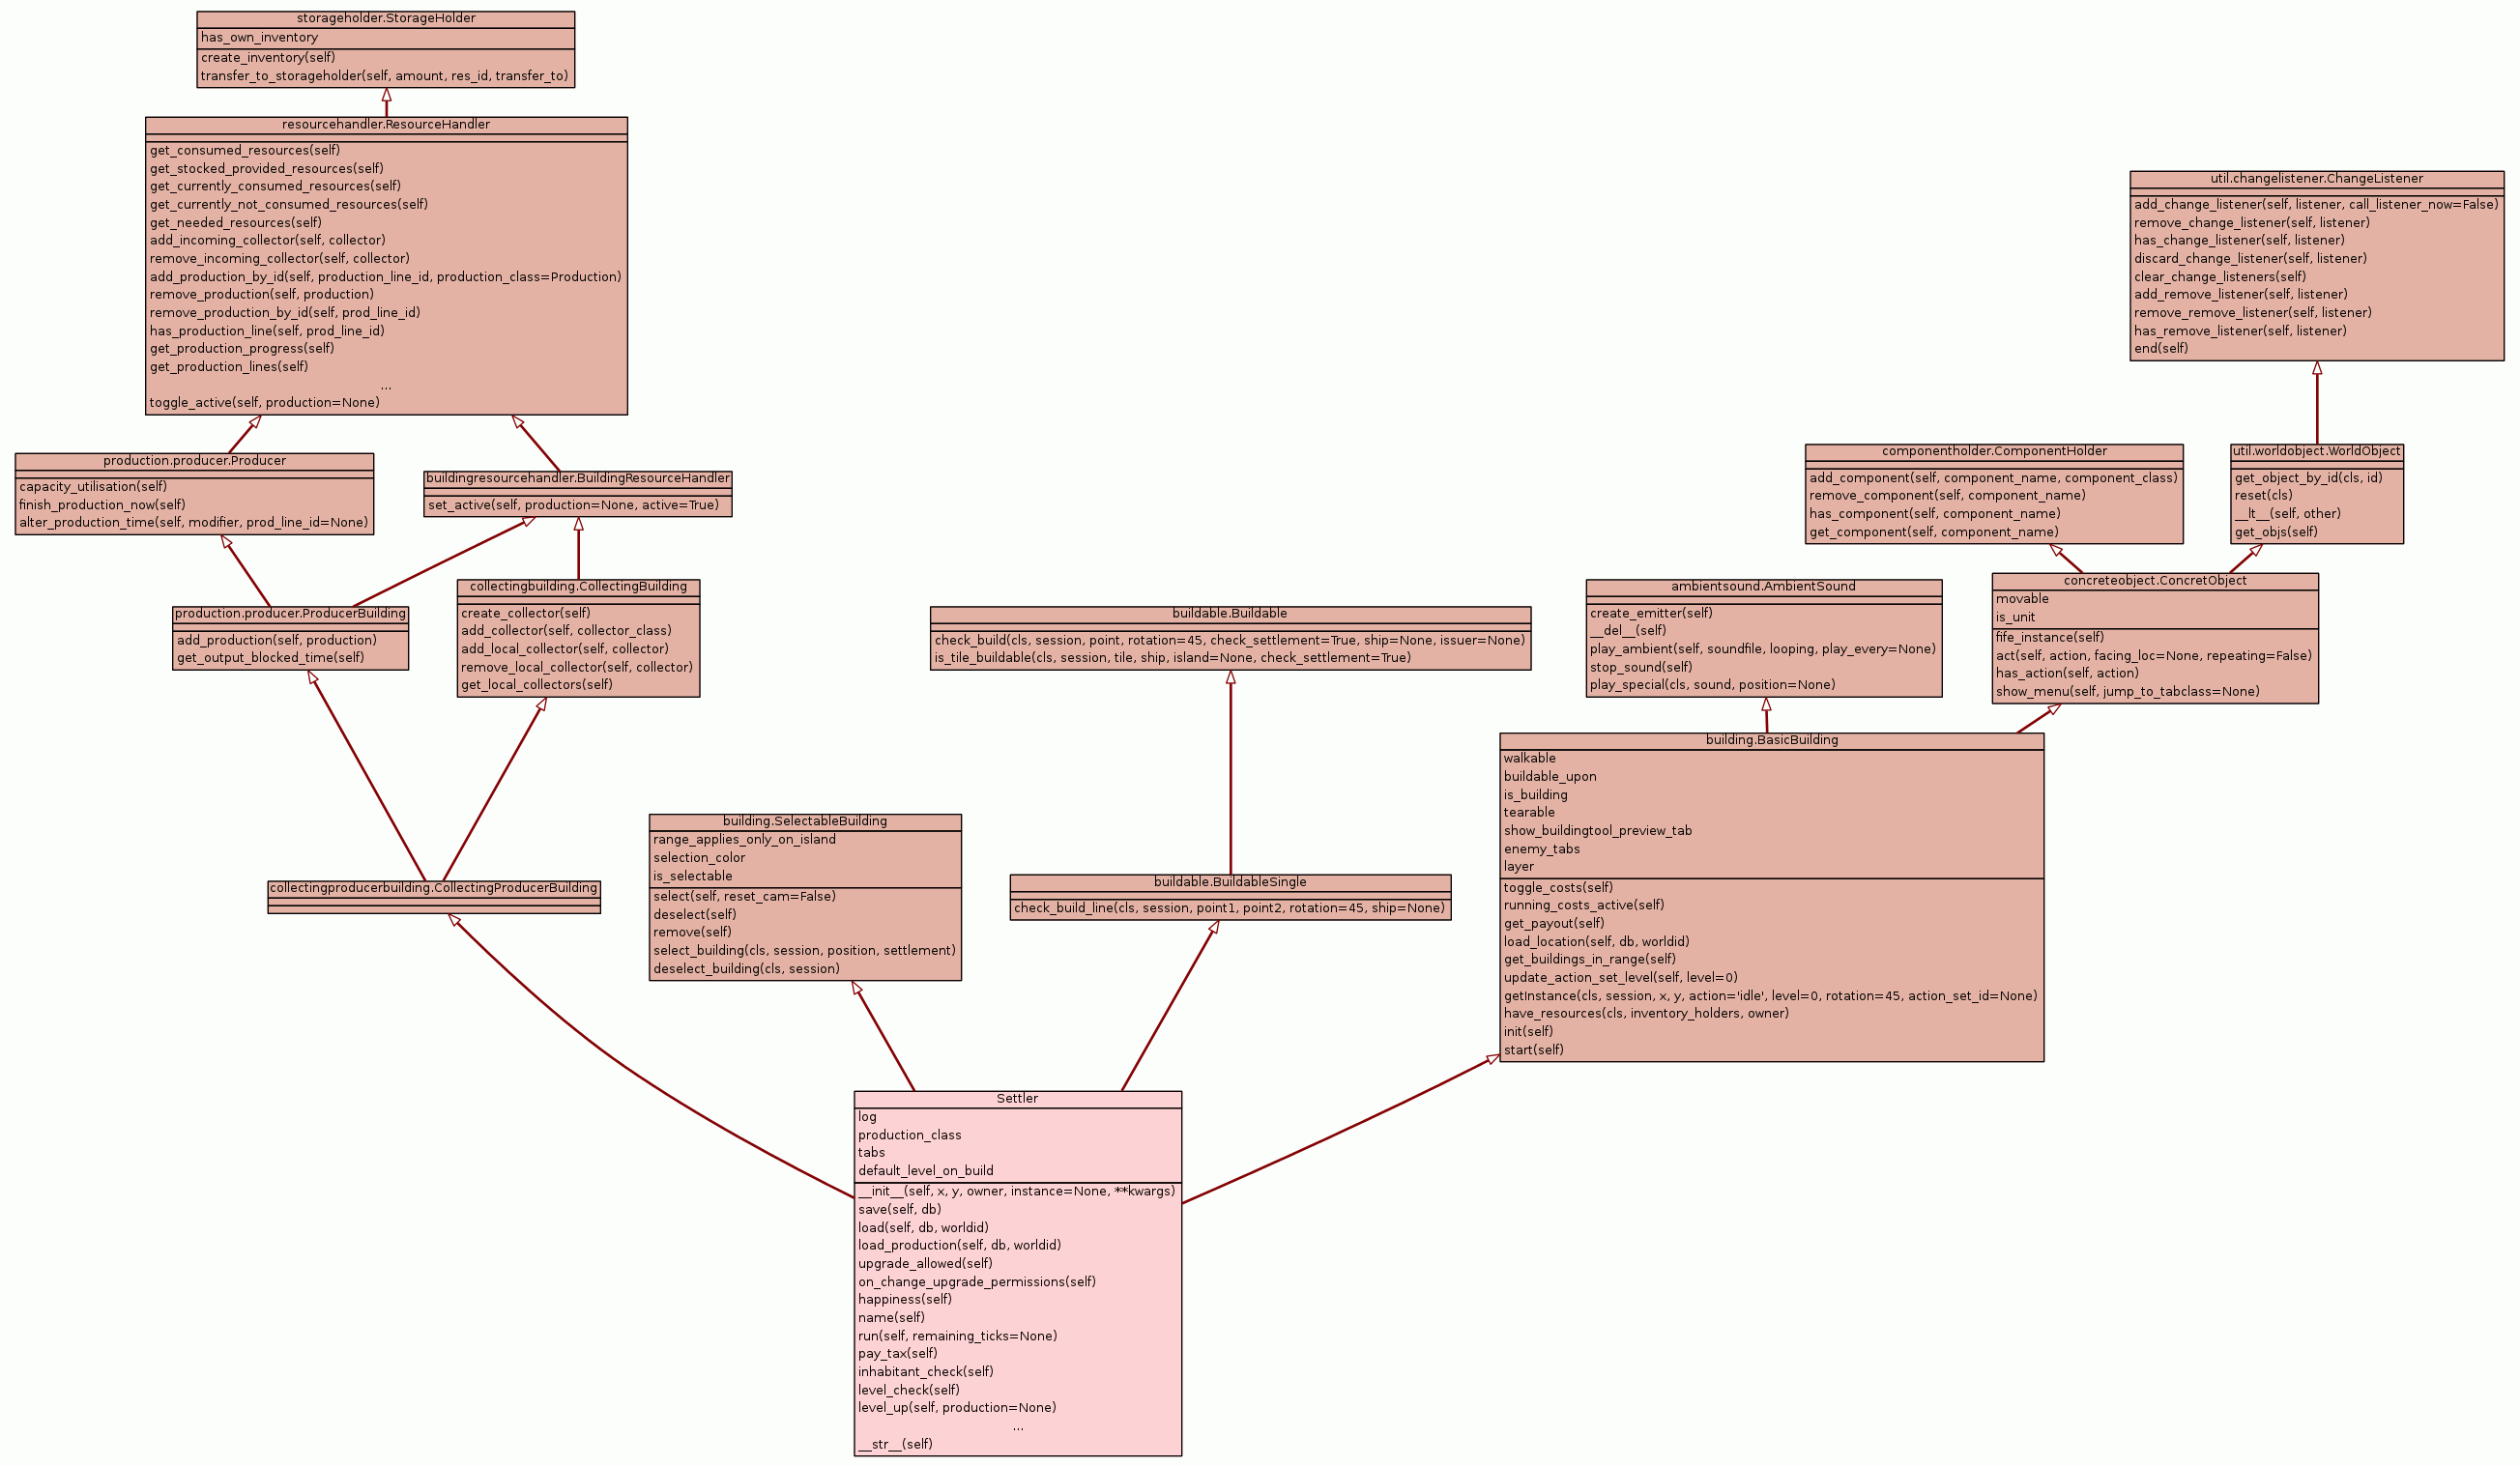
\includegraphics[angle=90,scale=0.25]{pics/settler_uml}
\caption{Inheritance tree for the \textit{Settler} class in \UH{}}
\label{fig:settleruml}
\end{figure}
The tree consists of 16 classes including many cases of multiple inheritance. 

Experience in working on this project has shown that making changes to any of the classes included in this tree is often
a very big task and comes with a great risk of introducing bugs into the code. It is also very difficult or even
impossible to write unit tests for these classes, as they are so dependent on each other and the game core, that it is
almost impossible to create the needed environment synthetically.

\paragraph{Settler Explained}
The \textit{Settler} class is comprised of 4 basic classes: \textit{BasicBuilding}, \textit{SelectableBuilding},
\textit{BuildableSingle} and \textit{CollectingProducerBuilding}. This is how most buildings in \textit{Unknown
Horizons} are constructed. 

\textit{BasicBuilding} is a base class for every building, it loads graphics and provides
basic information like the name, position, owner and functionality for running costs and level upgrades.

\textit{SelectableBuilding} is a decorating class, that implements functions for selecting the building ingame. It
manages showing ingame menus and outlines. If a building is not supposed to be selectable, this class should not be
inherited.

\textit{BuildableSingle} is a decorating class which is used when building new buildings. It tells the game that it can
only be built as single instance, so there is no building of multiple instances at once. For this purpose the code
provides the \textit{BuildableLine}, \textit{BuildableRect}, etc. classes which can be used if needed.

\textit{CollectingProducerBuilding} is a collectiv class to make the Settler have collecting units which pick up
resources for usage and then produce something from it. This is easier to demonstrate on a \textit{LumberJack} for
example, he picks up trees and produces planks from it. The Settler consumes resources (food, textiles, etc.) and in
turn produces the abstract resource happiness.

\paragraph{Datadriven?}
\UH{} uses a SQLite\footnote{SQLite website: \url{http://www.sqlite.org/}} to save parts of the object's
attributes. For example the size, health and name are saved in the database. This is necessary to make the highler level
classes in the architecture reusable for subclasses. All buildings have a size, but it may be different from building
type to building type. It is saved to an external file to make it easily editable by non programmers.

In summary we can say that the objects are partly datadriven, but usually it is not possilbe to add new buildings
without writing new code.

\subsubsection{RQ2}
In order to add a new building to \UH{} one has to look at the characteristics the building should have and
then find the appropriate classes from the \UH{} building classes collection. Those can then be combined to
form new buildings.

For example to create a settlement wall one could use the classes \textit{BuildableLine} and
\textit{BasicBuilding}. This is a very simple example which does not need to inherit many classes, as its functionality
is very limited. All attributes of this building can then be added in the database by using any SQLite database manager.

\subsubsection{RQ3}
Modifying existing ingame objects in \UH{} can be easy and very difficult. This depends on the degree of
change that is to be made. If only basic attributes like health, production time or similar are to be changed, then it
can easily be done by someone who knows their way around the database. If however new functionality is required, for
example an building which previously did not collect resources needs to collect resources, a change in the games code is
most certainly required. Again sometimes if the functionaliy exists, this can be easy by just adding another class to
the hierarchy of the building or it can be very difficult if new functionaliy in the existing classes is required.

A good example for this is the boatbuilder, which is mainly a \textit{CollectingBuilding} which produces units instead of
resources. The building has been implemented for over a year now and the team is still not certain if it works bugfree
or not, as it required huge modifications to the production classes to be able to produce units instead of resources.

\subsubsection{RQ4}
There are no tools available to help with the addition/edition of content at this point. A map editor is planned for
future versions, but it is not yet in a working state.


\subsection{Battle for Wesnoth}
\BOW{} as described on the project's website:
\begin{quote}
\textit{The Battle for Wesnoth is a Free, turn-based tactical strategy game with a high fantasy theme, featuring both
single-player, and online/hotseat multiplayer combat. Fight a desperate battle to reclaim the throne of Wesnoth, or take
hand in any number of other adventures... }
\end{quote}

\subsubsection{RQ1}
\subsubsection{RQ2}
\subsubsection{RQ3}
\subsubsection{RQ4}

\subsection{Mega Glest}
\GLEST{} as described on the project's website:
\begin{quote}
\textit{MegaGlest is a free and open source 3D real-time strategy (RTS) game, where you control the armies of one of
seven different factions: Tech, Magic, Egyptians, Indians, Norsemen, Persian or Romans. The game is setup in one of 16
naturally looking settings, which -like the unit models- are crafted with great appreciation for detail. Additional game
data can be downloaded from within the game at no cost.}
\end{quote}

\subsubsection{RQ1}
\GLEST{} uses a mixture of inheritance and component-based object description. Basic things are set using
inheritance, for example the \textit{UnitType} class inherits from the \textit{ProducibleType} class, as every unit in
the game is producable. More advanced things are added to the unit as components, for example the \textit{UnitType} has
\textit{Level},\textit{SkillType}, \textit{Resource}, \textit{CommandType} and \textit{UnitParticleSystemType}
components. Units themselves are part of a bigger compontent hierarchy: Units are part of a \textit{FactionType}, which
is part of a \textit{TechTree}. See \figref{LABEL} for a detailed structure analysis.
\textit{Map}

\subsubsection{RQ2}
\subsubsection{RQ3}
\subsubsection{RQ4}

\subsection{0 A.D.}

\subsection{Evaluation}

\subsection{Transferring the Results to \UH{}}
\subsubsection{Design}
\subsubsection{Implementation}
